\documentclass[12pt]{article}
% adjust style for page
\usepackage{fancyhdr}
% adjust the gap between content and margins of pages 
\usepackage{geometry}
% import images
\usepackage{graphicx} 
% tweak math elements
\usepackage{amsmath}
% import other .tex files into the main .tex
\usepackage{import}
% for simulating model content
\usepackage{lipsum}
% for hyper link that connects to other URL
\usepackage{hyperref}
% for tables having specific width
\usepackage{tabularx} 
% together used with "tabularx" package
\usepackage{booktabs}
% control position of elements precisely
\usepackage{float}
% control the caption element for table and figure
\usepackage{caption}
% for some math symbols and format
\usepackage{amsmath} % for 'cases' environment
% To manage footnotes in tables
\usepackage{threeparttable}  
% i forget the function of this one, GPT told me to include it :) 
\usepackage{babel}
% for multirows
\usepackage{multirow}
% for biblatex
% \usepackage[backend=biber]{biblatex}
% for hyper link
\usepackage{hyperref}

\newenvironment{myfigure}[3] % width, path, caption
{
    \begin{figure}[htbp]
        \centering
        \includegraphics[width=#1\textwidth]{#2}
        \caption{#3}
}
{
    \end{figure}
}

\title{
Assignment 2 of STAT5320
}

\author{Feng Gu(T00751197), Anti Li(T00751339), Yuzhuo Ye(T00751492)}
% \date{\today}

\begin{document}
\maketitle

\section{Preamble}
\subsection{Declaration of Using Generative Artificial Intelligence}
The ideas and work are designed by the authors, with the use of ChatGPT in some parts of coding and grammar checking.

\subsection{Support Materials for This Assignment}
All relevant code and results are stored in the GitHub repository:

\href{https://github.com/Gufeng-2002/5320_assignment_2.git}
{\textit{Click here to access the repository.}}

\subsection{Solid text less than 3 pages}
We have checked that after moving all tables and figures to the appendix, the main text is less than 3 pages.


\section{Explore the relationship between X's and Y's}

Before we build the linear model with MLE method, we can explore the relationship
between X's and Y's by plotting the scatter plot.

The figure \ref{fig:anscombe_quartet} shows the scatter plot of Anscombe's 4 different 
data set.

\begin{figure}[!h]
    \centering
    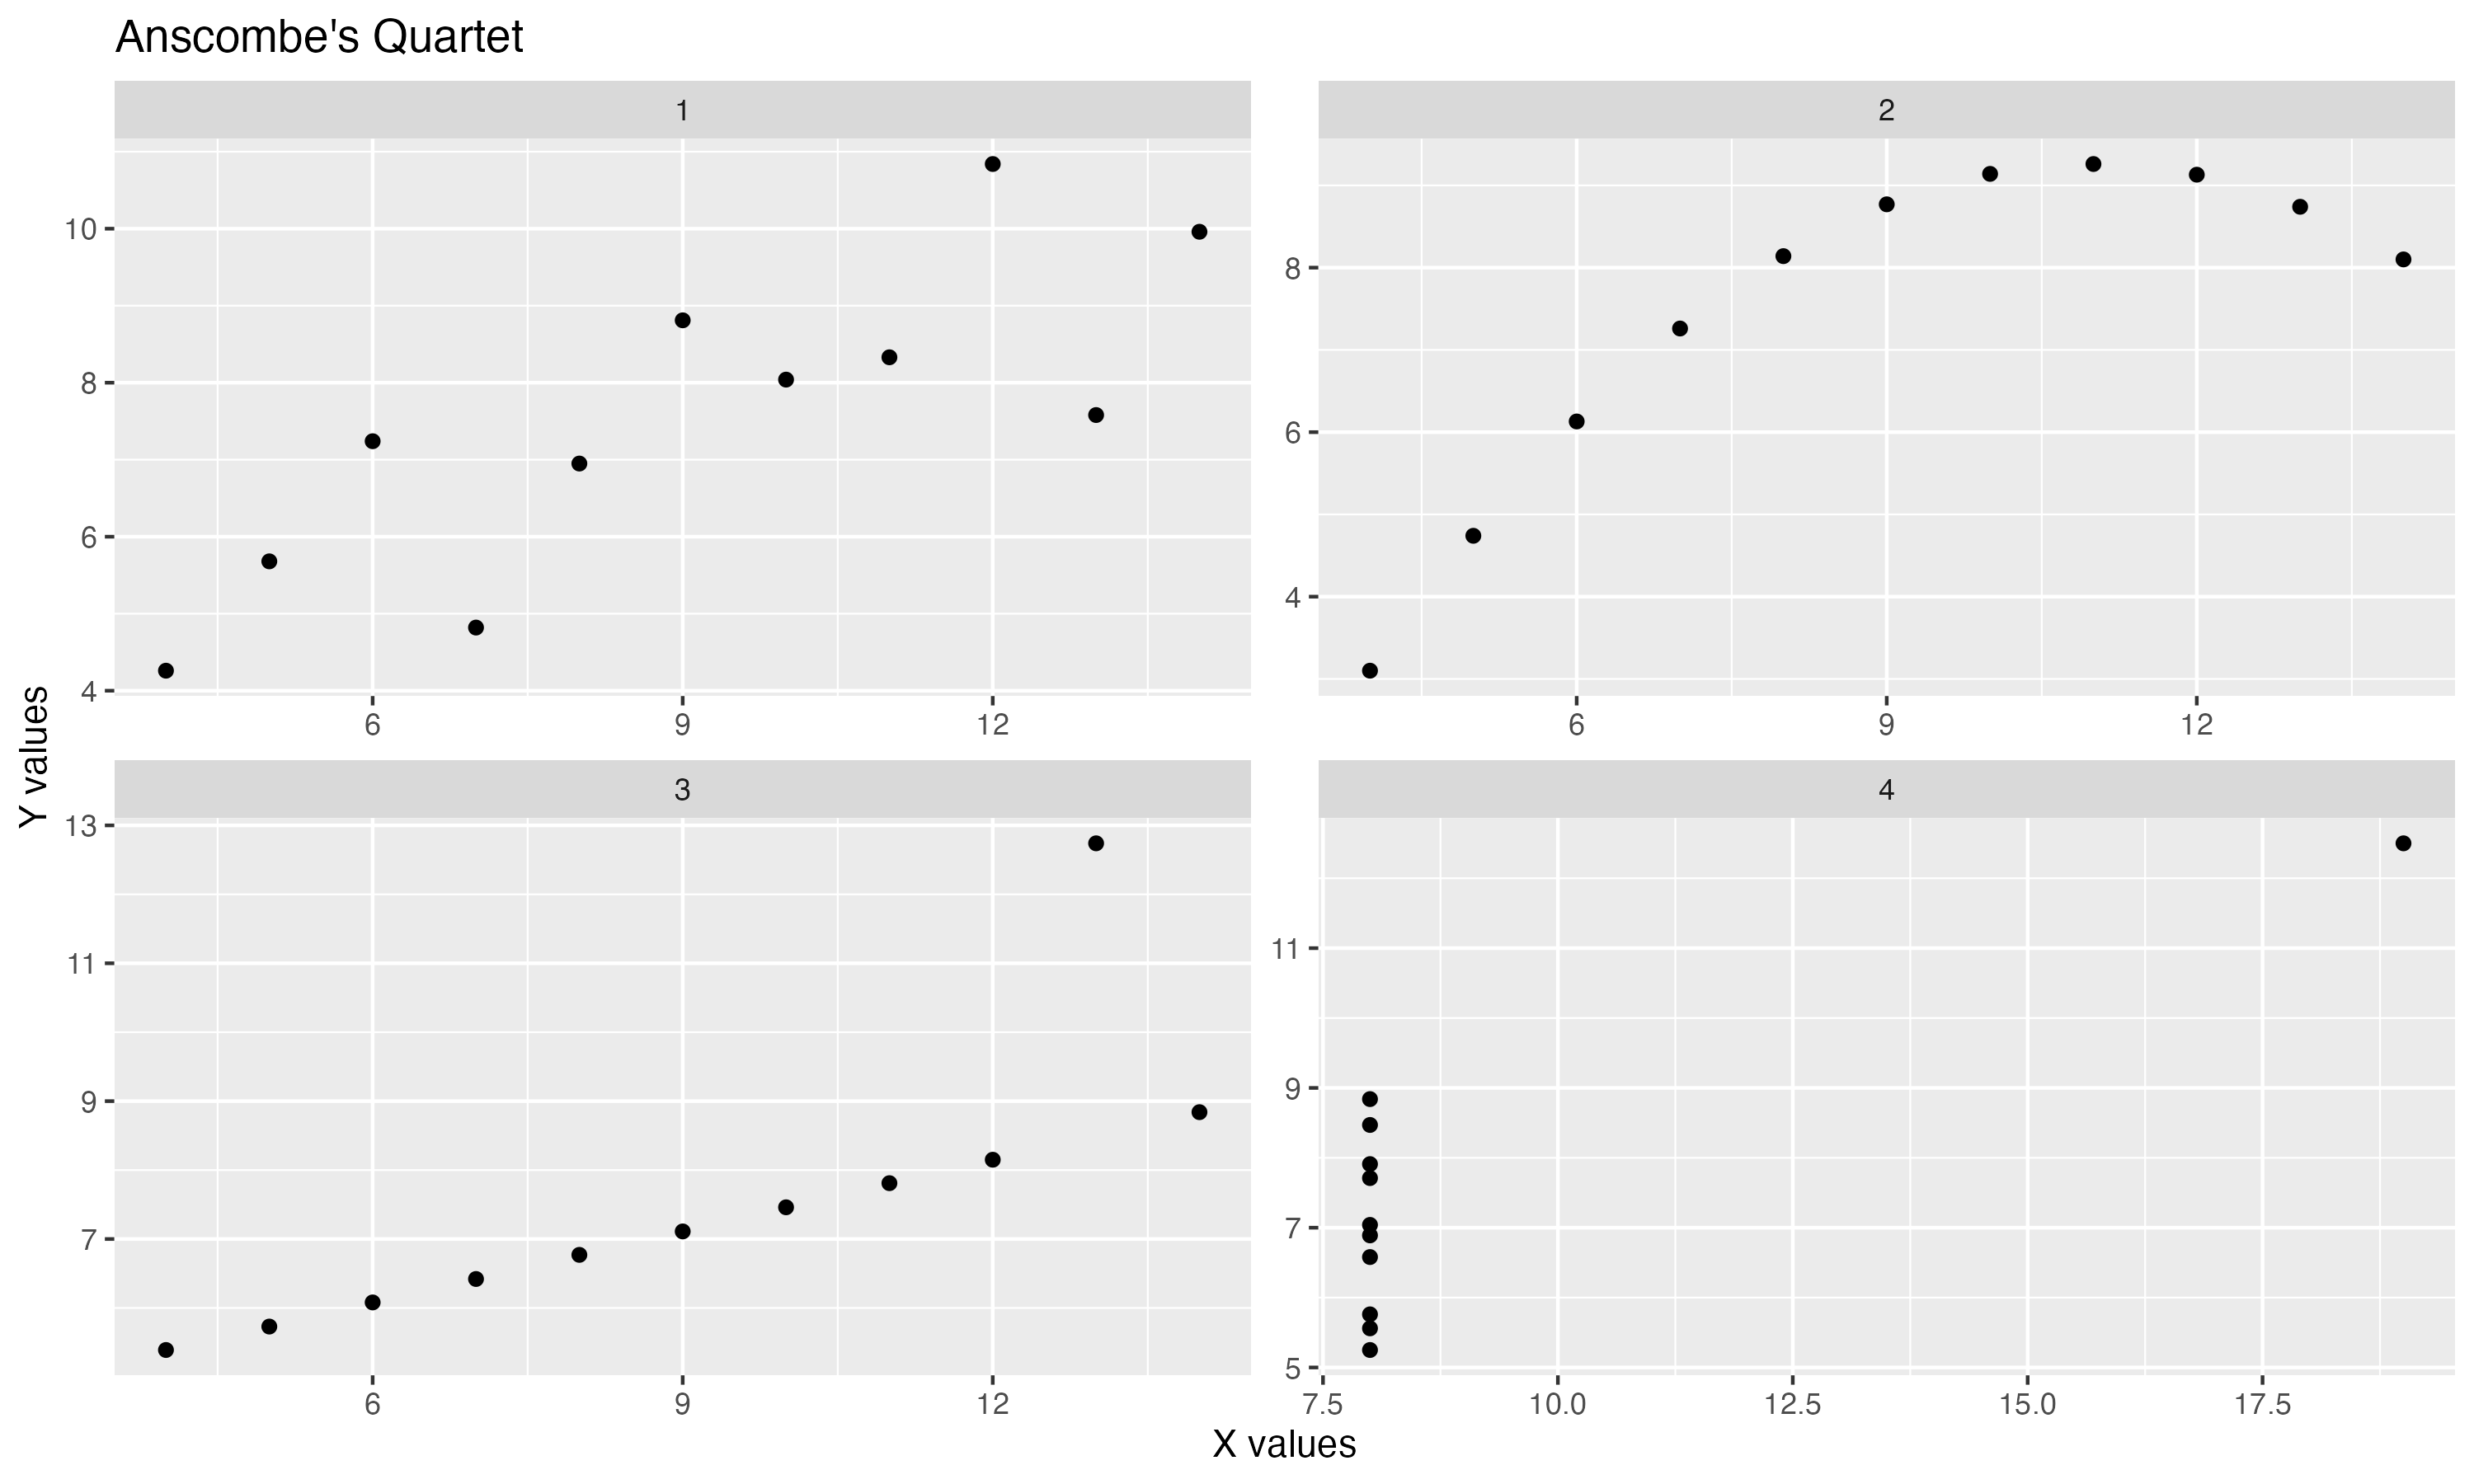
\includegraphics[width=0.9\textwidth]{../results/anscombe_quartet.png}
    \caption{Anscombe's Quartet}
    \label{fig:anscombe_quartet}
\end{figure}

Based on the scatter plot, it is suitable to build linear models for some of the data sets, 
but others are not. Let us build simple linear models for each of them with MLE in estimating
the coefficients.

\section{Fit a linear model to each dataset}

\subsection{What the MLE method results are supposed to be}
In each data set, we assume \(X\) probabilistically determines \(Y\) by assume the following:
\[
Y = \beta_0 +\beta_1 X + \epsilon, \quad \epsilon \sim N(0, \sigma^2)
\]

Given a data set, we can estimate the coefficients by maximizing the log-likelihood function,
assuming \(X's\) and \(\epsilon's\) are 'iid'.
\[
argmax_{\beta_0, \beta_1} \sum_{i=1}^{n} \log f(y_i | x_i, \beta_0, \beta_1)
\]

If our assumption about the model and distribution of \(\epsilon\) is correct,
the residuals should be normally distributied with mean 0 and constant variance 
\(\sigma^2\) on each level of \(X\).

% latex table generated in R 4.4.1 by xtable 1.8-4 package
% Sun Mar  9 16:15:36 2025
\subsection{Model Fitting Results}
The table \ref{tab:model_fitting_results} shows the linear coefficients, p-values for each data set with the MLE method we set in 
the previous section.

\begin{table}
  \centering
  \begin{tabular}{llrrrrr}
    \hline
  model & term & coefficients & std\_errors & t\_values & p\_values & $R^2$ \\ 
    \hline
  \multirow{2}{*}{data 1} & $\beta_0$ & 3.00 & 1.12 & 2.67 & 0.03 & \multirow{2}{*}{0.67} \\ 
    & $\beta_1$ & 0.50 & 0.12 & 4.24 & 0.00 &  \\ 
    \hline
  \multirow{2}{*}{data 2} & $\beta_0$ & 3.00 & 1.13 & 2.67 & 0.03 & \multirow{2}{*}{0.67} \\ 
    & $\beta_1$ & 0.50 & 0.12 & 4.24 & 0.00 &  \\ 
    \hline
  \multirow{2}{*}{data 3} & $\beta_0$ & 3.00 & 1.12 & 2.67 & 0.03 & \multirow{2}{*}{0.67} \\ 
    & $\beta_1$ & 0.50 & 0.12 & 4.24 & 0.00 &  \\ 
    \hline
  \multirow{2}{*}{data 4} & $\beta_0$ & 3.00 & 1.12 & 2.67 & 0.03 & \multirow{2}{*}{0.67} \\ 
    & $\beta_1$ & 0.50 & 0.12 & 4.24 & 0.00 &  \\ 
     \hline
  \end{tabular}
  \caption{Model Fitting Results} 
  \label{tab:model_fitting_results}
\end{table}
From the regression results, we found that all models have the same coefficients and \(R^2\) value, 
even though the relationship between X's and Y's are different in each data set(shown in fig \ref{fig:anscombe_quartet}).

The figure \ref{fig:anscombe_quartet_fitted} shows the fitted lines for each data set. We found the lines are the same but 
the relationship between X's and Y's are not always linear.

\begin{figure}[!h]
    \centering
    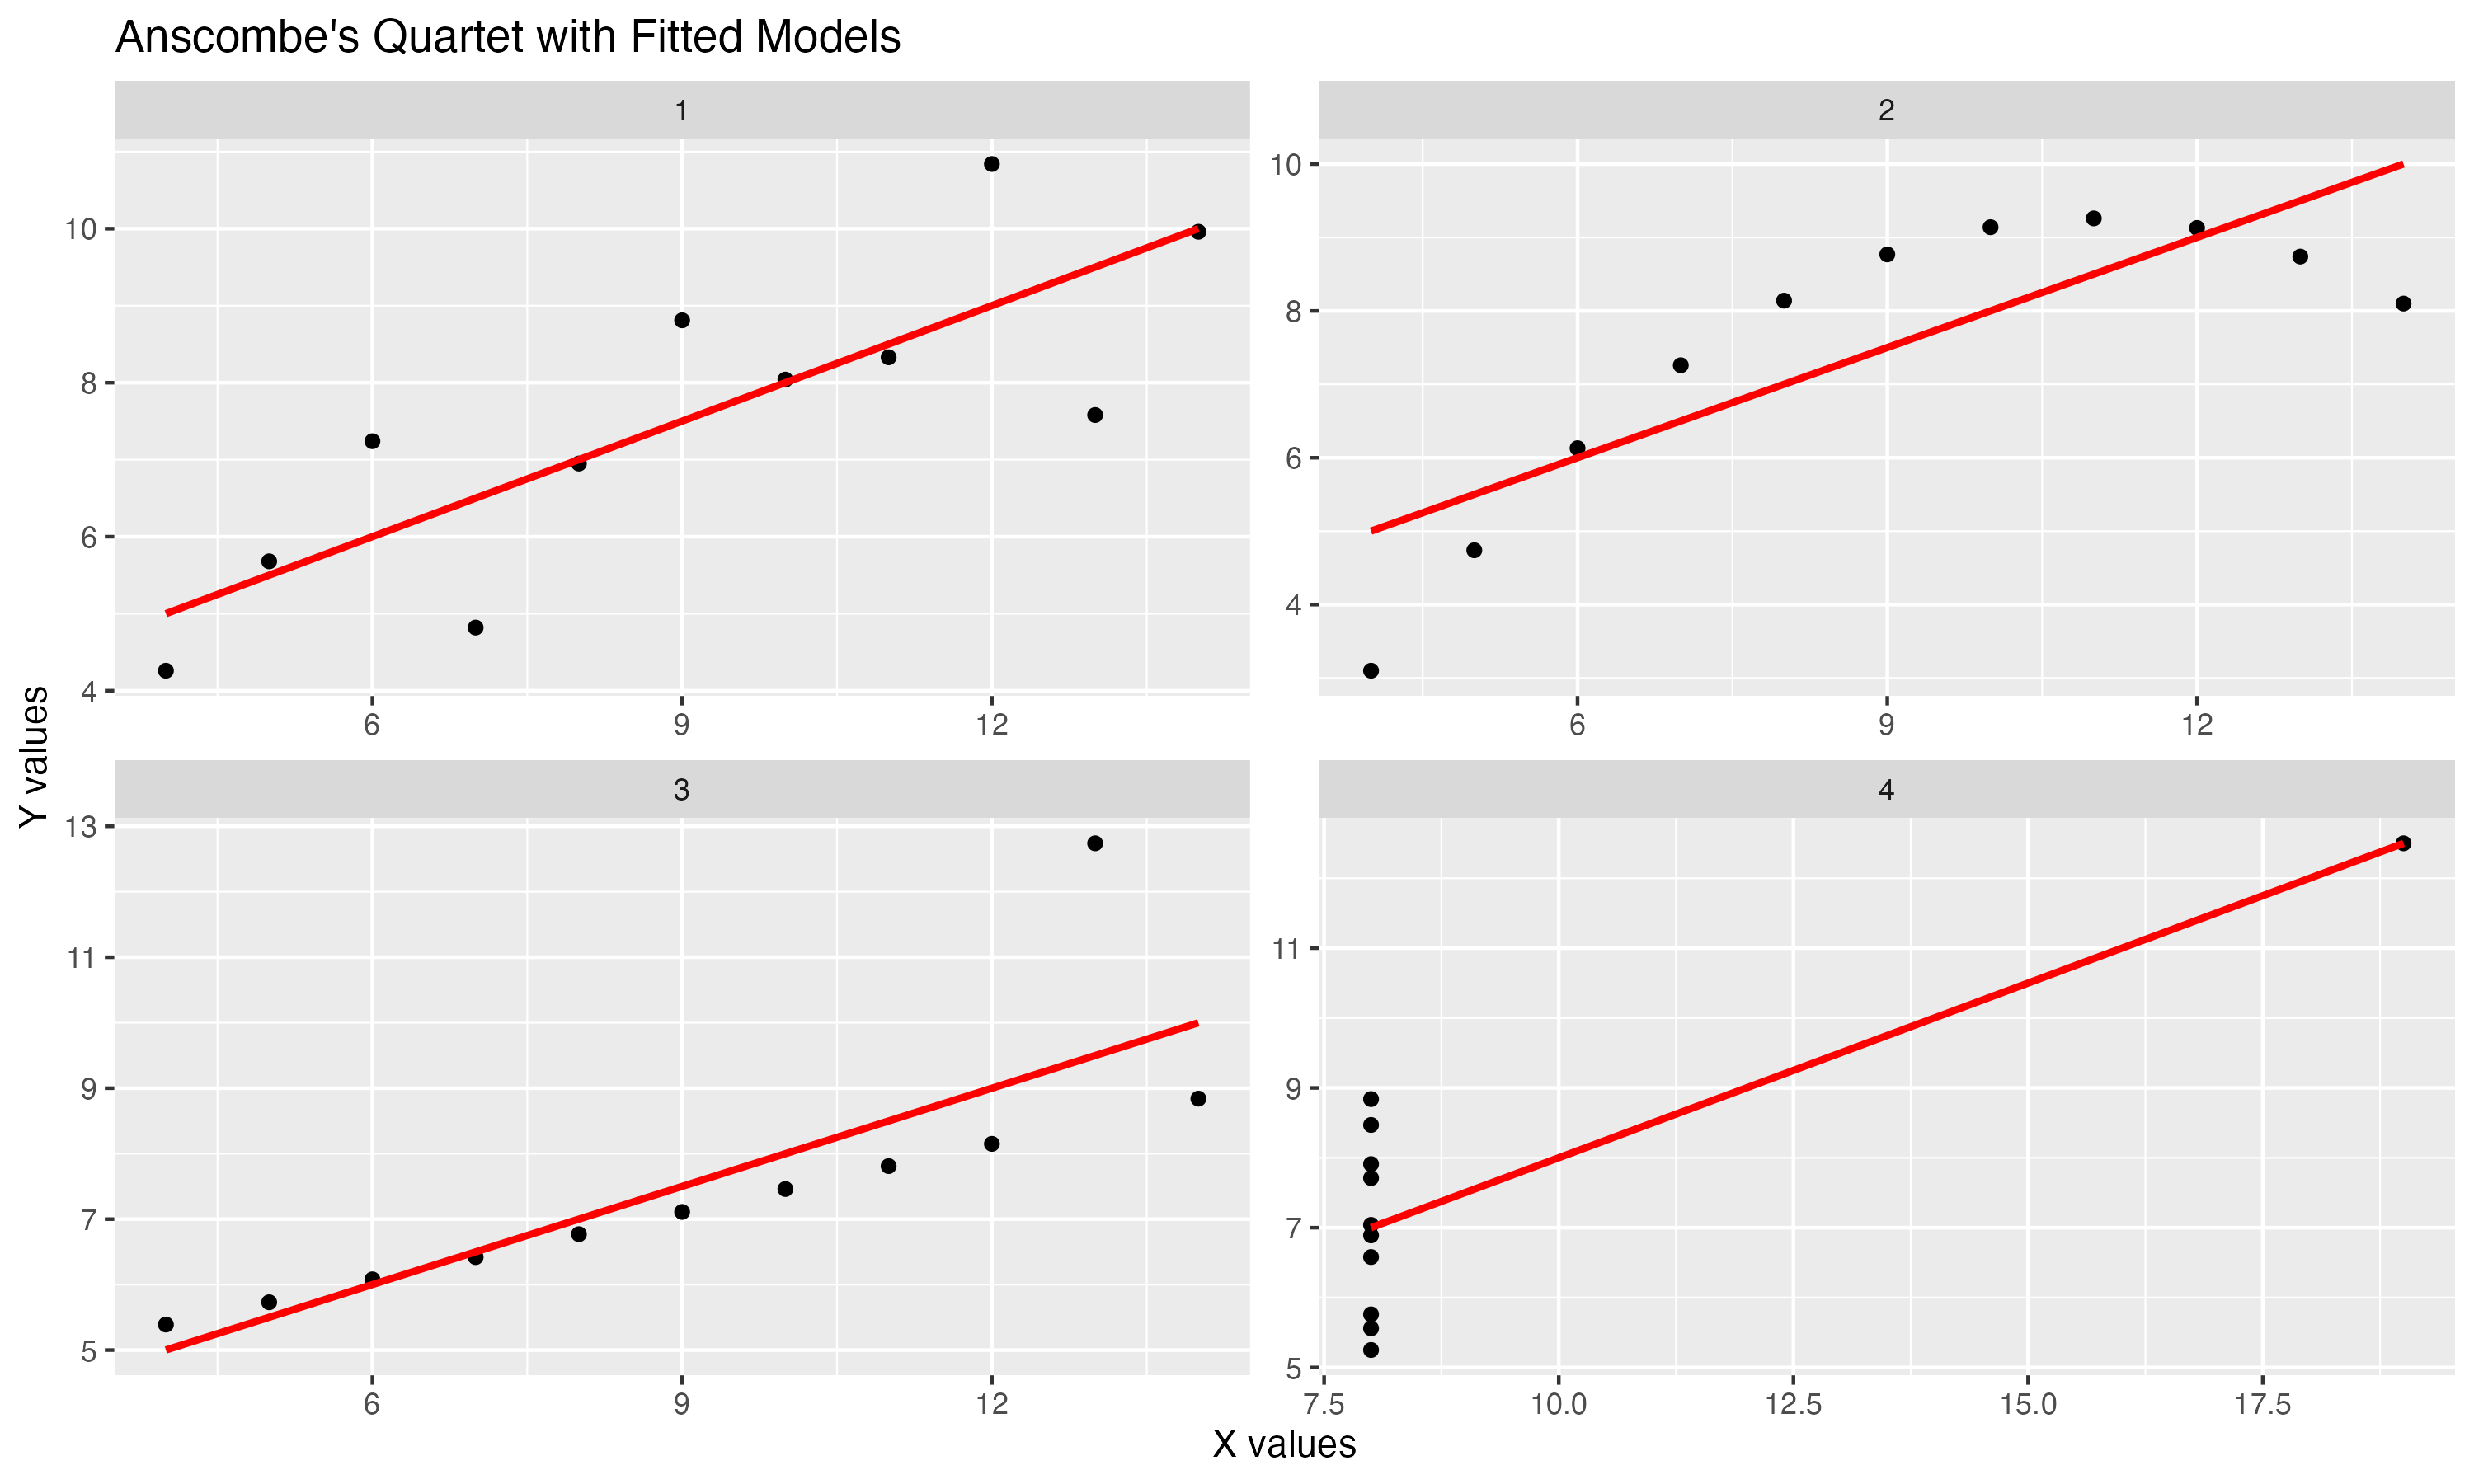
\includegraphics[width=0.9\textwidth]{../results/anscombe_quartet_fitted.png}
    \caption{Anscombe's Quartet with Fitted Lines}
    \label{fig:anscombe_quartet_fitted}
\end{figure}

\section{Residual Analysis for each data set}
According to the assumption we made in the MLE method, if the residuals distri-bution were correctly spcified, 
the distribution of residuals from the models should be normal with mean 0 and constant variance \(\sigma^2\), on each
level of \(X\), due to \(\epsilon_i \overset{iid}{\sim} N(0, \sigma^2)\).

We draw the residuals against each fitted values(which are corresponding to levels of \(X\)), 
the histogram of residuals and Q-Q plot of residuals for each data set, shown in figures \ref{fig:residuals_vs_fitted}, 
\ref{fig:residuals_histogram}(appendix) and \ref{fig:residuals_qq}.

\begin{figure}
    \centering
    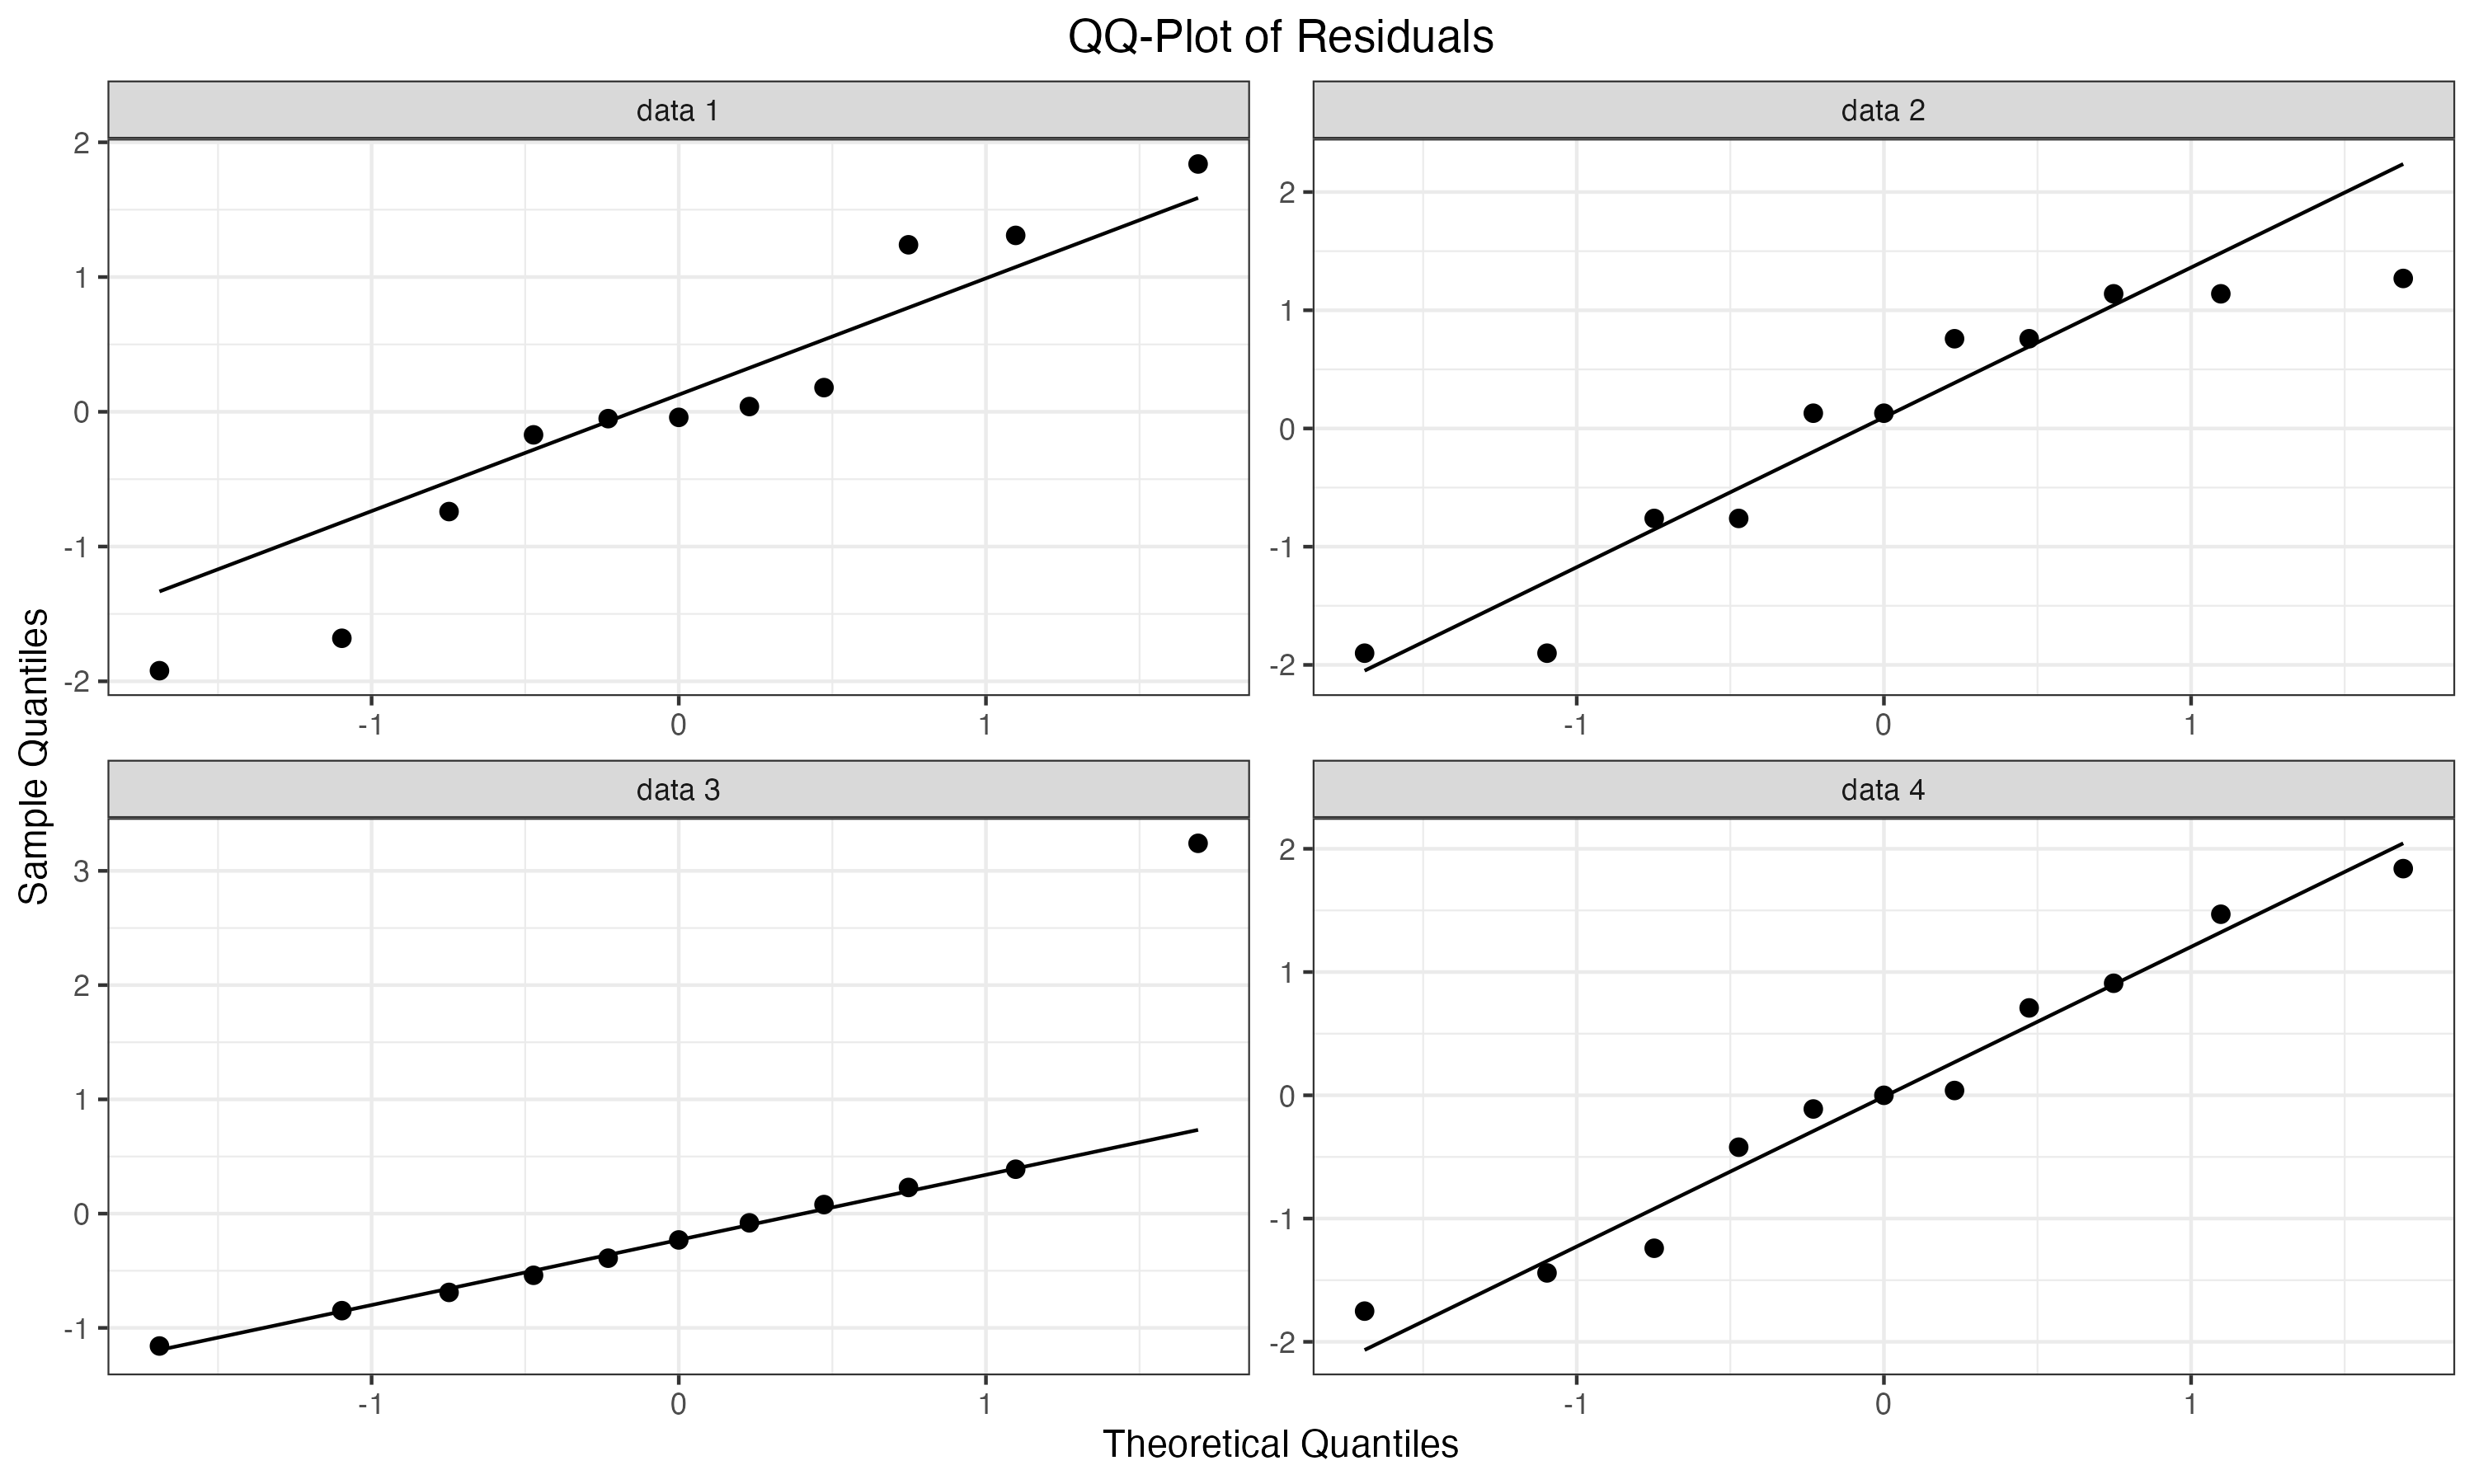
\includegraphics[width=0.9\textwidth]{../results/residuals_qq.png}
    \caption{Q-Q Plot of Residuals}
    \label{fig:residuals_qq}
\end{figure}

From these residual distribution plots, if we believe that these \(\epsilon_i\) 
exhibit homo-scedasticity with \(E(\epsilon_i) = 0\), and they
come from the same distribution, and are independent, we found that the residuals 
are not exactly normally distributed.

\begin{itemize}
  \item For data set 1:
  
       The residuals exhibit a slight right skewness, indicating they are not perfectly normally distributed. 
       However, this residual distribution is acceptable.
  \item For data set 2:
       The residuals have a heavy right tail, 
       indicating that residuals are more likely to have higher values.
  \item For data set 3:
       The residuals appear very close to a normal distribution, 
       but there is one extreme outlier in the regression, which affects the normality.
  \item For data set 4:
       The residuals appear closest to a normal distribution,
        but all except one are from a single level of \(X\), 
        which is not ideal for establishing the relationship between \(X\) and \(Y\). 
\end{itemize}

\section{What we can glean about model fits from the residuals}

From the simple linear models we built for each data set, it is clear that
even though the relationship between X's and Y's can be different in levels of X, or 
the residuals distribution properties are different, we can still get the same coefficients and 
\(R^2\) value for them. 

\textbf{Personally speaking, part of this problem might be caused by the assumption that \(\epsilon_i\) are 'iid'.} This assumption
determines that all residuals are from a same distribution, regardless of the levels of X and the true relationship
between X and Y.
It casues that we equally consider each observation with the same weight and apply this regression relationship to other levels.
However it should not be the trueth in real world.

Except the assumptions about reisudals, \textbf{the correct setting about the par-tially deterministic relationship between X and Y is 
also crucial in model-ing.} Reviewing back to what we have fitted for data set 2(fig \ref{fig:anscombe_quartet_fitted}), the relationship between \(X\) and \(\hat Y\)
should be quadratic rather than linear. But we still use linear pattern to capture this relationship, which is lack of capability to capture the true relationship, 
causing the \(R^2\) not high enough.


\clearpage
% Bibliography section
\begin{thebibliography}{99} % The number specifies the width of the label

  \bibitem{example1}
  H. Hyndman and G. Athanasopoulos. 
  ``STL Decomposition,'' 
  \textit{Forecasting: Principles and Practice (3rd ed.)}. 
  Available at: \url{https://otexts.com/fpp3/stl.html}. 
  Accessed: November 30, 2024.

\end{thebibliography}

\section{Appendix}

\begin{figure}[!h]
  \centering
  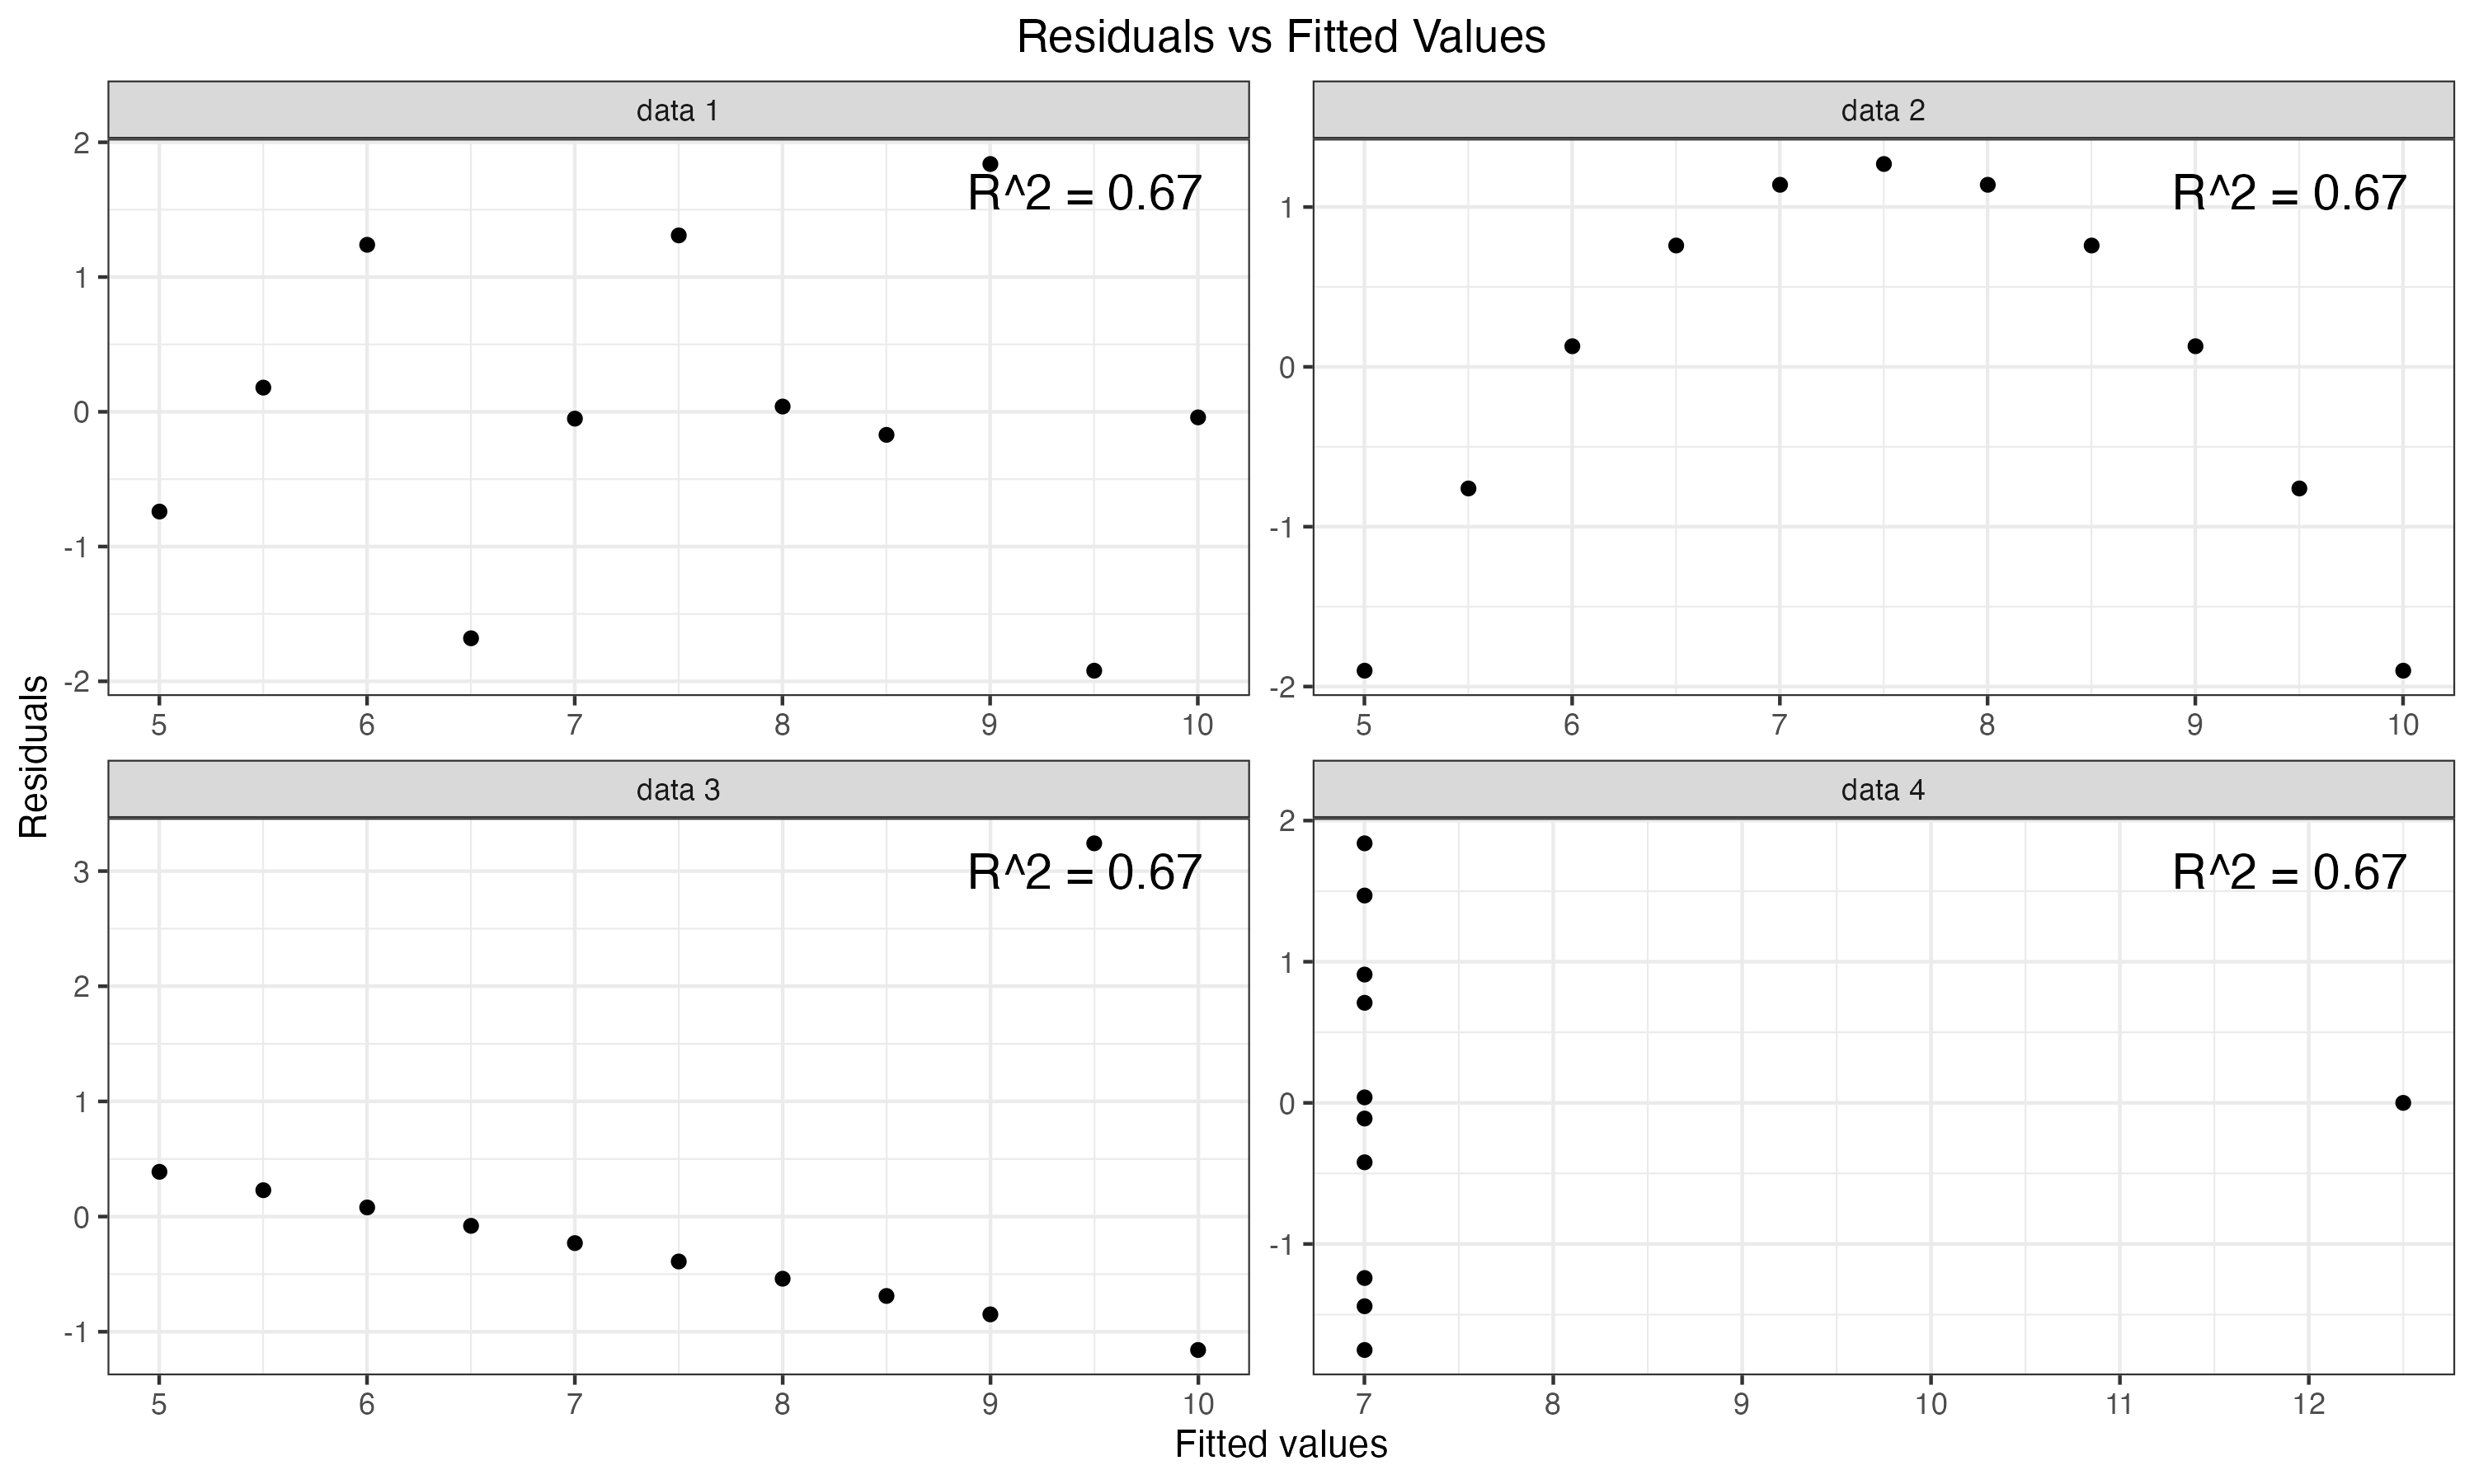
\includegraphics[width=0.9\textwidth]{../results/residuals_vs_fitted.png}
  \caption{Residuals vs Fitted Values}
  \label{fig:residuals_vs_fitted}
\end{figure}

\begin{figure}[!h]
  \centering
  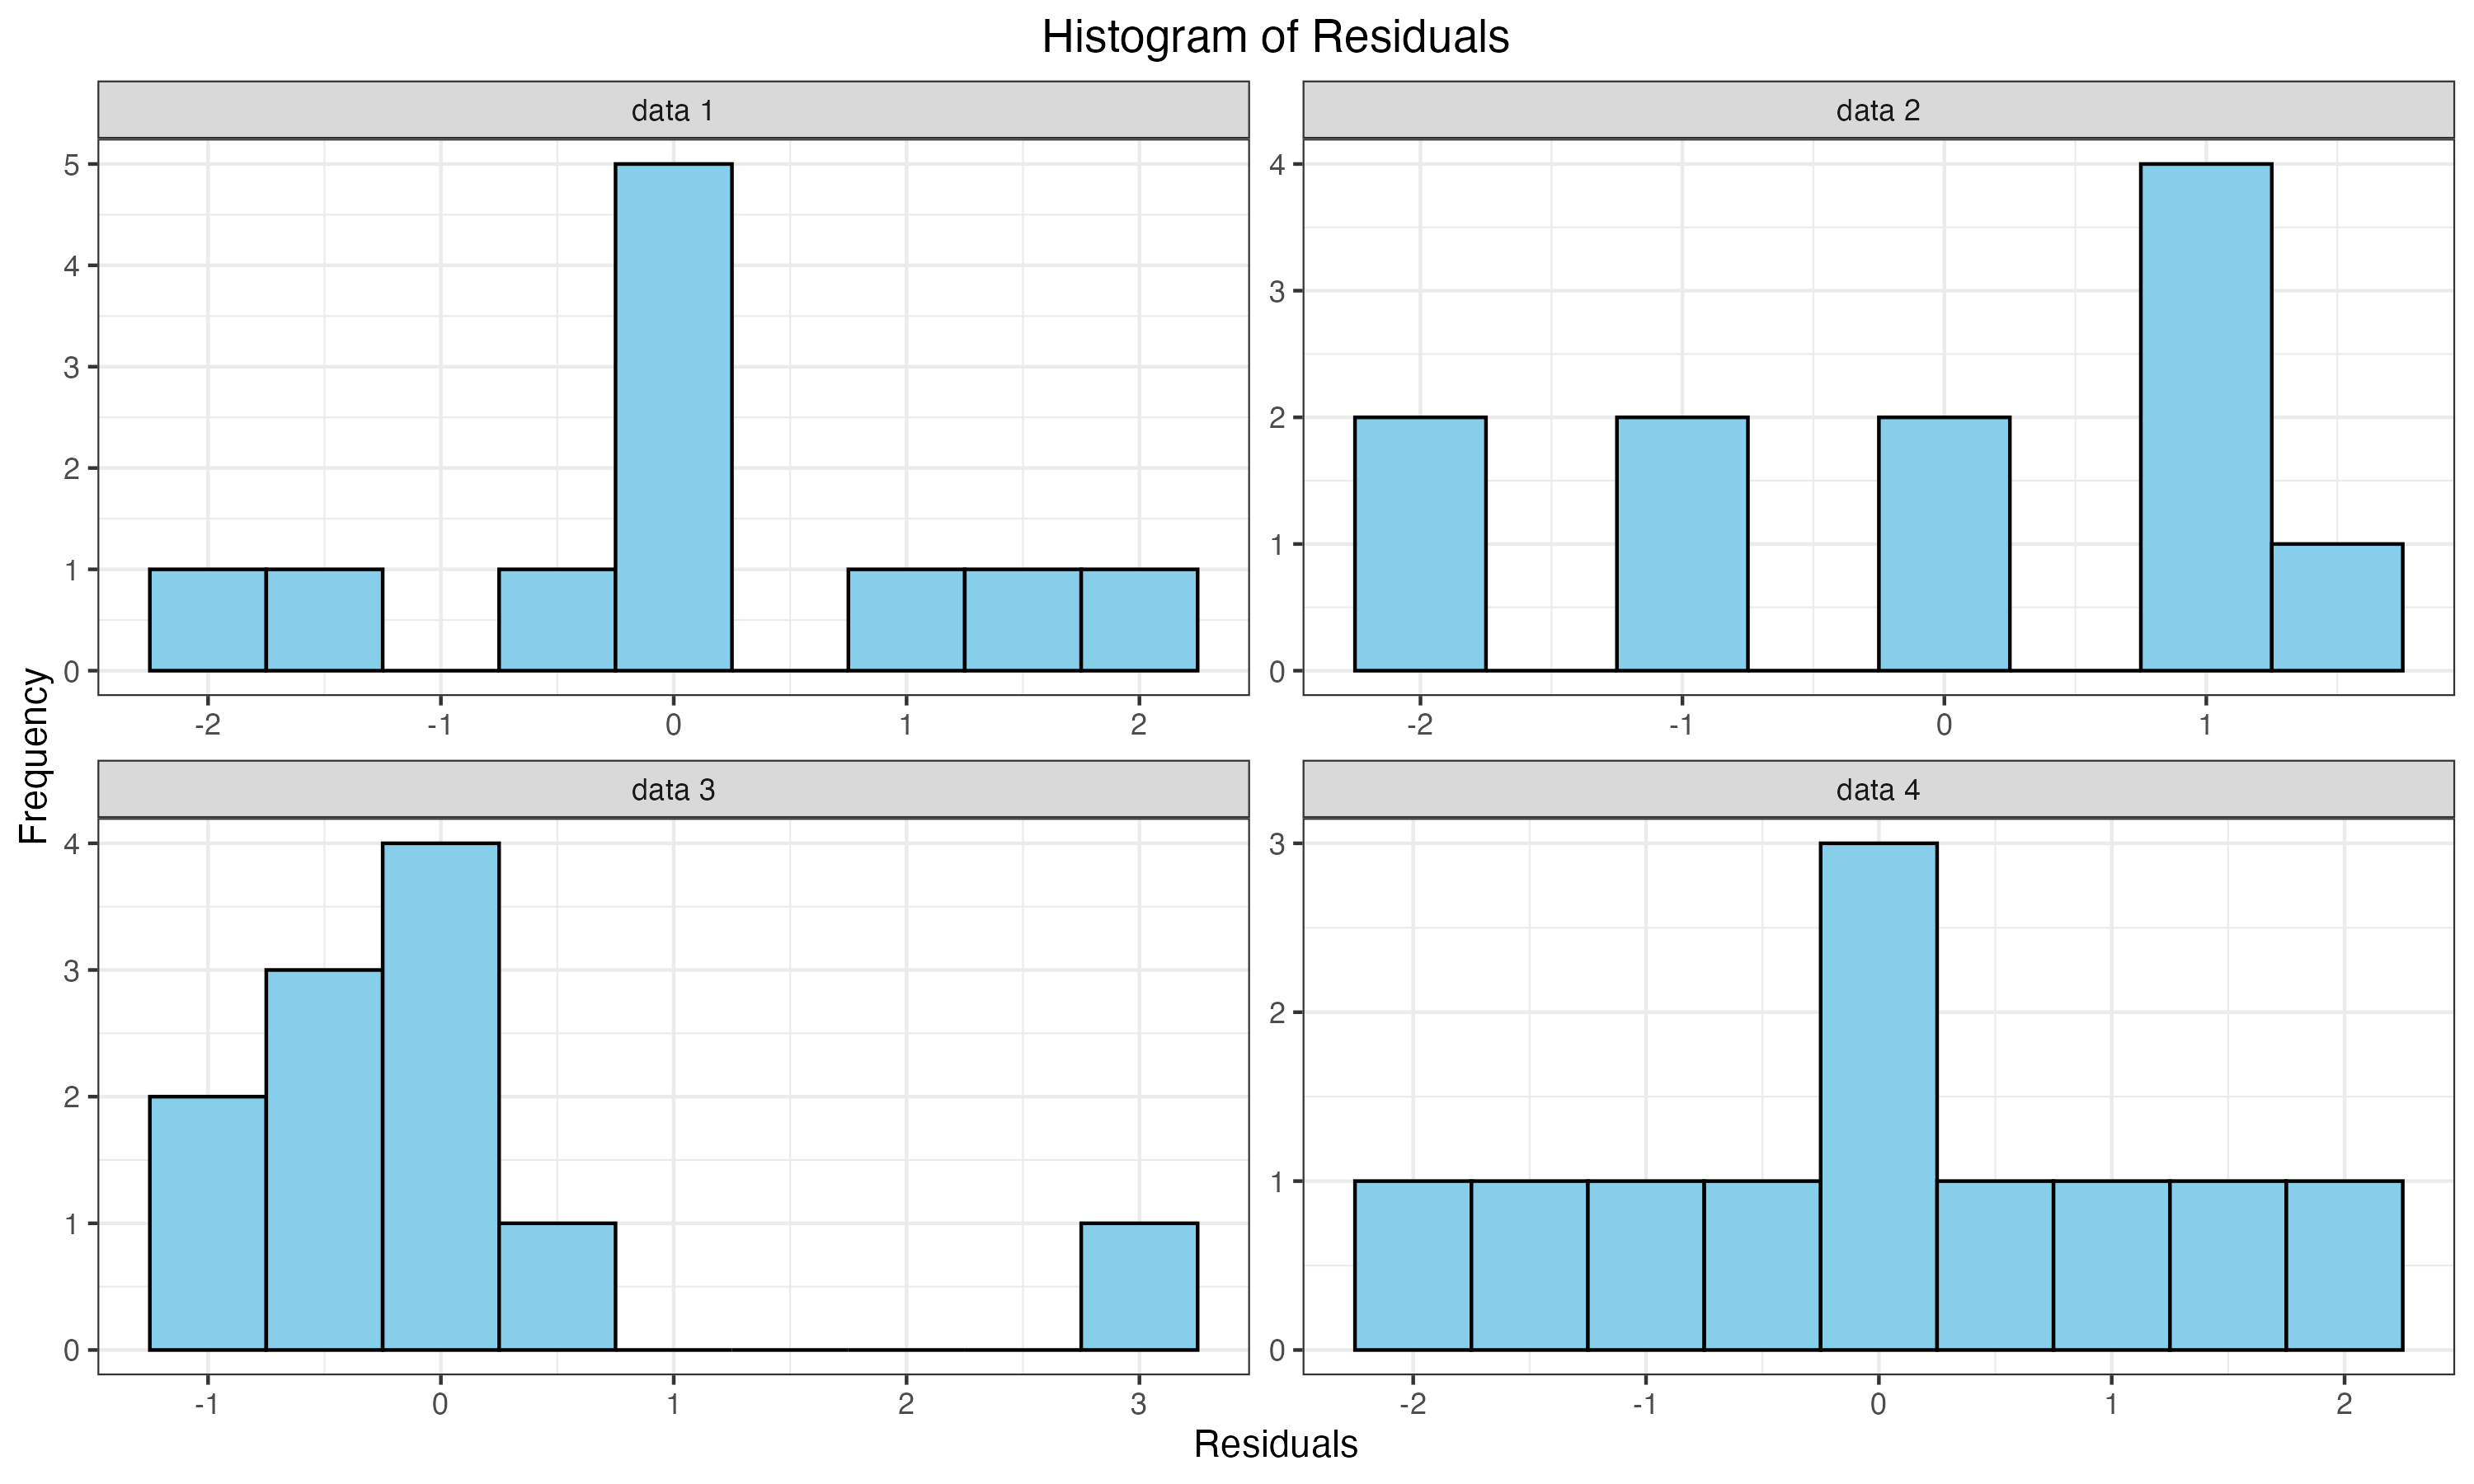
\includegraphics[width=0.9\textwidth]{../results/residuals_histogram.png}
  \caption{Histogram of Residuals}
  \label{fig:residuals_histogram}
\end{figure}

\end{document}
